
\documentclass{article}
\usepackage{color}
\usepackage{amsmath}
\usepackage{subcaption}
\captionsetup{compatibility=false}
\usepackage{graphicx}
\usepackage{grffile}
\usepackage{epstopdf}
\begin{document}



\section{Model predictive control unconstrained}

\subsection{UAV dynamics}
For understanding the UAV's controller, it is important to understand the physical properties of UAV. It has 4 rotors, 


\subsection{MPC Introduction}
MPC is an advanced regulator, using prediction of future states of the system for determining system input actions. Because of it's computational demanding, it is used mainly in processes with long time constants, such as control of chemical processes. Using MPC for controlling UAV is a big challenge, because it is hard to implement on embedded hardware. 
The MPC needs to know the system's state space model, initial condition and, unlike other controllers, a sequence of desired future states. Another great advantage of MPC is applying large variety of constraints. On the other hand, MPC is sensitive to the model inaccuracy and to errors in input. Output of the MPC is not only desired input actions in next time step, but also predicted action inputs in the whole prediction horizon for T following time steps. 

\subsection{Formulation of quadratic programming}
MPC formulates optimization problem, that then has to be solved. The problem takes form of Linear Programming(LP), or in this case Quadratic Programming(QP). 

\begin{equation}
\label{eq:QP_formulation}
\begin{split}
\mathrm{V}\left(\textbf{\underline{x}}, \textbf{\underline{u}}\right) = \frac{1}{2}\sum_{i=0}^{M-2}\left(\textbf{e}^T_{[i]}\textbf{Q}\textbf{e}_{[i]} + \textbf{u}^T_{[i]}\textbf{P}\textbf{u}_{[i]}\right) + \frac{1}{2}\textbf{e}_{[M-1]}\textbf{S}\textbf{e}_{[M-1]}
\end{split}
\end{equation}


There are several ways to solve this problem, which will be discussed later.





\subsection{Coordinate system}
This whole problem will be solved in 2D only. The height of the UAV is controlled separately. There are several reasons to do that. The first one is, that most applications use constant height, for example building interiors. The desired trajectory is usually also given in 2D. The second reason is, as mentioned above, MPC is very demanding on computing time. To save computational capacity, standard PID controller can be used instead. The height PID controller has already been implemented and it is will not be part of this thesis. In these 2 dimensions, there are 2 axis as shown in {\color{red}figure...}. There are two coordinate systems, which will be used. The first one is a standard world coordinate system W. The second one is a coordinate system U, which is a system with origin in the UAV. Coordinate system U is created only by translation of the system W for the vector $\vec{r} = (\Delta x, \Delta y)$. There is no rotation between the two coordinate systems, so the axis of the both coordinate systems are parallel. Because the UAV can move easily along each axis, there is no need to introduce the UAV's rotation. If the UAV would rotate over time, the model would no more be linear and control of this system would be much more complex. These coordinate systems transformations work according the equation \ref{eq:coordinate_transform}.

\begin{equation}
\label{eq:coordinate_transform}
\begin{split}
x^{(W)} = x^{(U)}+\Delta x	\\
y^{(W)} = y^{(U)}+\Delta y	\\
\dot{x}^{(W)} = \dot{x}^{(U)}+\Delta \dot{x}	\\
\dot{y}^{(W)} = \dot{y}^{(U)}+\Delta \dot{y}	\\
\ddot{x}^{(W)} = \ddot{x}^{(U)}+\Delta \ddot{x}	\\
\ddot{y}^{(W)} = \ddot{y}^{(U)}+\Delta \ddot{y}	\\
\end{split}
\end{equation}

In the following text, there will be used the world coordination system W unless stated otherwise.

\subsection{One axis model}
% picture of UAV
The UAV model has been already analyzed --cite Tomas--. Thanks to symmetrical body of the UAV, both axis have the same model. For one axis, the states take form of 
$\vec{x}_x = (x_x; \dot{x}_x; \ddot{x}_x)^T$ and $\vec{x}_y = (x_y; \dot{x}_y; \ddot{x}_y)^T$, where $x_x$ is the aileron and $x_y$ is the elevator position. The aileron and elevator models are mathematically identical. The system in discrete state space model takes form of system matrices $\textbf{A}_s, \textbf{B}_s$ according to equation \ref{eq:state_space_model_simple}

\begin{equation}
\label{eq:state_space_model_simple}
\vec{x}_{x,y,[t+1]} = \textbf{A}_{x,y} \vec{x}_{x,y, [t]} +\textbf{B}_{x,y} u_{x,y, [t]}
\end{equation}

where $u_{x,y,[t]}$ is an input at time $t$, sampling with the frequency of $1/\Delta t = 70Hz$.




\begin{equation}
\textbf{A}_{x,y} =
  \begin{bmatrix}
  1 & \Delta t & 		0 \\
  0 & 		 1 & \Delta t \\
  0	& 		 0 &		p_1
  \end{bmatrix},\textbf{B}_{x,y} = \begin{bmatrix}
  0 \\
  0 \\
  p_2
  \end{bmatrix}, 
\end{equation}

where $p_1 = 0.9799$ and $p_2 = 5.0719\cdot10^{-5}$. The unconstrained MPC can be computed separately for elevator and aileron axis. Simple constraints, such as input saturation can be applied.

\subsection{{\color{red} Linked/Extended} model}		% extended?
For more complex constraints, such as position constraints, one axis position is a function of the other axis position. For these kinds of constraints more complicated system is needed. The state space system must be preserved, connecting both identical systems for each axes into one system extending equation \ref{eq:state_space_model_simple} into 

\begin{equation}
\label{eq:state_space_model_simple}
\textbf{x}_{[t+1]} = \textbf{A} \textbf{x}_{[t]} +\textbf{B} \textbf{u}_{[t]}
\end{equation}

where $\textbf{u}_{[t]} = (u_{x,[t]}, u_{y,[t]})^T$ is input vector containing elevator and aileron system inputs at the time $t$. Extended state vector $\textbf{x}_{[t]} = (x_{[t]}, \dot{x}_{[t]}, \dot{x}_{[t]}, y_{[t]}, \dot{y}_{[t]}, \ddot{y}_{[t]})^T$ contains positions $x,y$ and theirs derivatives at the time $t$. 

By connecting these 2 systems, we get the following state space matrices of the whole system
\begin{equation}
\label{eq:state_space}
\begin{bmatrix}
	\textbf{A}_s & \textbf{0}	\\
	\textbf{0}   & \textbf{A}_s
\end{bmatrix}, \textbf{B} = \begin{bmatrix}
	\textbf{B}_s & \textbf{0}	\\
	\textbf{0}   & \textbf{B}_s
\end{bmatrix}.
\end{equation}



\subsection{Kalman}
As mentioned in introduction, MPC is very sensitive to noise and errors. Wrong initial condition can result in a bad prediction because of the double integration of acceleration into position. To work properly, the MPC has to have access to very accurate initial condition. These measurements are position, speed and acceleration in both axis. An Kalman estimator has been already implemented -cite Tomas- to estimate all states of the UAV. Above all of that, it estimates disturbances of the acceleration.

%% Hovd, Morten. "A brief introduction to Model Predictive Control." URL= http://www. itk. ntnu. no/fag/TTK4135/viktig/MPCkompendium% 20HOvd. pdf (2004).




\subsection{system constraints}
One of the greatest advantages of MPC is being able to apply large variety of constraints. As mentioned in \ref{eq:QP_formulation}, the MPC uses linearly constraint quadratic programming for finding the input action prediction. The constraints must defined with the matrices $\textbf{A}_c$ and $\textbf{B}_c$ according to 

\begin{equation}
\textbf{A}_cu<\textbf{B}_c
\end{equation}

$\textbf{A}_c$ is a matrix of width 2T and height of the number of constraints applied. $\textbf{B}_c$ is a column vector of the same height.

\subsubsection{input constraints}
In control, one of the biggest problems one must overcome is system saturation. This means, that the real system is linear only on a certain range of inputs and can't achieve desired output \cite{saturation}. For example motor can spin in certain maximum speed despite input voltage. Also, if the controller sends too high input actions, the system can be destroyed. This can happen for example in PD control, when the difference between real and desired output changes rapidly in time, for example because of sensory noise.
The standard  solution for this kind of problem is simply saturate the output of the controller. This is a very simple solution, but it is not the best one. Because the controller doesn't know about this saturation, the system will not behave correctly.
The great advantage of input constraints in MPC is, that the controller will consider these aspects of real system and find an input prediction, that will not violate the constraints and at the same time will achieve the desired output. 

% graphs of saturated controllers:
%		1) MPC with only saturated inputs
%		2) MPC with saturated outputs
%		3) PID with saturated outputs

\begin{figure}[tbp]
\centering

\begin{subfigure}[b]{0.55\textwidth}
	\includegraphics[width=\textwidth]{fig/step_constrained_2.eps}
	\caption{Tricopter aircraft.}
	\label{fig:tricopter}
\end{subfigure}%
\begin{subfigure}[b]{0.45\textwidth}
	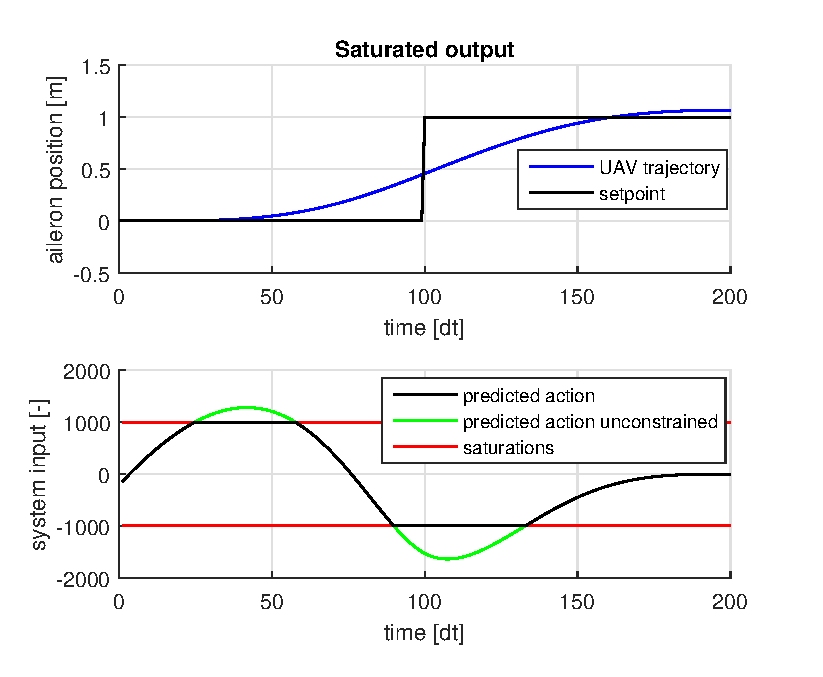
\includegraphics[width=\textwidth]{fig/step_saturated_2.eps}
	\caption{The px4flow sensor.}
	\label{fig:px4flow}
\end{subfigure}

\caption{Tricopter platform with px4flow optical flow sensor.}
\label{fig:tricopter_px4flow}
\end{figure}

The condition 

\subsubsection{}

\subsection{System prediction}
The MPC algorithm is based on predicting future states based on initial condition and system input. Such a general equation must be found. Let's repeat the equation \ref{eq:state_space_model_simple}.

\begin{equation}
\textbf{x}_{[t+1]} = \textbf{A}\textbf{x}_{[t]} + \textbf{B}\textbf{u}_{[t]},
\label{eq:mpc_lti_system}
\end{equation}

With a simple substitution we can get prediction of the states at the time $t = 2$.

\begin{equation}
\begin{split}
\label{eq:mpc_lti_system2}
\textbf{x}_{[1]} &= \textbf{A}\textbf{x}_{[0]} + \textbf{B}\textbf{u}_{[0]},\\
\textbf{x}_{[2]} &= \textbf{A}\textbf{x}_{[1]} + \textbf{B}\textbf{u}_{[1]}\\
&= \textbf{A}\cdot(\textbf{A}\textbf{x}_{[0]} + \textbf{B}\textbf{u}_{[0]}) + \textbf{B}\textbf{u}_{[1]} \\
&=\textbf{A}^2\textbf{x}_{[0]} + \textbf{A}\textbf{B}\textbf{u}_{[0]} + \textbf{B} \textbf{u}_{[1]}
\end{split}
\end{equation}

The equation \ref{eq:mpc_lti_system2} can be rewritten in a more general way:

\begin{equation}
\label{eq:mpc_lti_system_general}
\textbf{x}_{[t]} =\textbf{A}^t\textbf{x}_{[0]} + 
\sum_{i = 1}^{t-1}\textbf{A}^{i}\textbf{B}\textbf{u}_{[i-1]} + \textbf{B} \textbf{u}_{[t-1]}
\end{equation}

Let's combine the sequence of predicted states into one vector $\textbf{\underline{x}} = (\textbf{x}_{[1]}^T, \textbf{x}_{[2]}^T, ..., \textbf{x}_{[T]}^T)^T$ and the sequence of inputs into 
$\textbf{\underline{u}} = (\textbf{u}_{x,[0]}, \textbf{u}_{y,[0]}, \textbf{u}_{x,[1]}, \textbf{u}_{y,[1]}, ..., \textbf{u}_{x,[T-1]}, \textbf{u}_{y,[T-1]})^T$
With this notation, equation \ref{eq:mpc_lti_system_general} can be represented as a simple matrix multiplication.

\begin{equation}
\label{eq:prediction_big}
\underbrace{
\begin{bmatrix}
\textbf{x}_{[1]} \\
\textbf{x}_{[2]} \\
\vdots \\
\textbf{x}_{[T]} \\
\end{bmatrix}}_{\textbf{\underline{x}}}
=
\underbrace{
\begin{bmatrix}
\textbf{A} \\
\textbf{A}^2 \\
\vdots \\
\textbf{A}^{(T-1)} \\
\end{bmatrix}}_{\textbf{\^A}}
\textbf{x}_{[0]}
+
\underbrace{
\begin{bmatrix}
\textbf{B} & \textbf{0} & \textbf{0} & \textbf{0} \\
\textbf{AB} & \textbf{B} & \textbf{0} & \textbf{0} \\
\vdots & \vdots & \ddots & \vdots \\
\textbf{A}^{(T-1)}\textbf{B} & \textbf{A}^{(T-2)}\textbf{B} & \hdots & \textbf{B}
\end{bmatrix}
}_{\textbf{\^B}}
\cdot
\underbrace{
\begin{bmatrix}
\textbf{u}_{[0]} \\
\textbf{u}_{[1]} \\
\vdots \\
\textbf{u}_{[T-1]} \\
\end{bmatrix}}_{\textbf{\underline{u}}}
\end{equation}

Using the new notation, this can be be rewritten in a simple form

\begin{equation}
\label{eq:prediction_final}
\textbf{\underline{x}} = \textbf{\^A}\textbf{x}_{[0]} + \textbf{\^B}\textbf{\underline{u}}.
\end{equation}

\section{Problem formulation}
As mentioned in a section ???, MPC uses a quadratic optimization problem. Let's first solve the problem, where obstacles are not involved. 
\subsection{Trajectory}
For every task, there is given a desired trajectory $\textbf{\underline{x}}_d = 
(\textbf{x}_{d,[1]}^T, \textbf{x}_{d,[2]}^T, ..., \textbf{x}_{d,[T]}^T)^T$, where the desired state at the time $t$ is $\textbf{x}_{d,[t]} = (x_{d,[t]}, \dot{x}_{d,[t]}, \ddot{x}_{d,[t]}, y_{d,[t]}, \dot{y}_{d,[t]}, \ddot{y}_{d,[t]})^T$. These desired states contain, besides aileron and elevator position, also velocity and acceleration. This gives the MPC a chance to  enforce other properties outside position. However, The UAV desired velocity is already given by the desired positions at certain time as the distance $d = \sqrt{(x_{d,[t]}-x_{d,[t+1]})^2+ (y_{d,[t]}- y_{d,[t+1]})^2}$ . The same can be applied for acceleration. Therefore, the velocity and acceleration is demanded in the sequence of desired positions, rather than the the states. The desired velocity and acceleration is than ignored, which will be discussed in a section ??? and it can hold any value, for example 0. The $\textbf{x}_{d,[t]}$ than takes form of $\textbf{x}_{d,[t]} = (x_{d,[t]}, 0, 0, y_{d,[t]}, 0, 0)^T$. When creating the desired trajectory, one should always keep in mind, that the desired positions hold also information about velocity and acceleration. 

\subsubsection{Objective function}
The goal of unconstrained MPC is to follow the given trajectory as well as possible. This means, that we want to minimize the error between all the predicted positions and the desired positions, gaining error:
\begin{equation}
\begin{split}
\label{eq:simple_err}
e_{x, t} = x_{[t]} - x_{d, [t]}\\
e_{y, t} = y_{[t]} - y_{d, [t]}
\end{split}
\end{equation}
Using this kind of error has many downsides. The first one is, that if we want to minimize it, we would have to take the absolute value. However this function would not be differentiable. The second one is, that we don't get very good  results if penalizing the error linearly. From the experience, it has come beneficial in many ways to use the the the square of the error. This preserves the condition of not prioritizing one direction error. The function is also easily differentiable. The next great advantage is penalizing big distances disproportionately more and ignoring very small errors. 
If a simple sum of $e_{x, t}^2$ and $e_{y, t}^2$ was applied, the system would behave very wildly, generating very high input actions to correct the error. However, this is not in the capabilities of the real system and could result in an unstable control. Therefore input actions must be penalized also. This combined together, we get the following objective function 

\begin{equation}
\label{eq:qmpc_basic_formulation}
% mala chyba, x nezahrnuje x0.
\mathrm{V}\left(\textbf{\underline{x}}, \textbf{\underline{u}}\right) 
= \frac{1}{2}\sum_{i=1}^{T}\left( k_q \cdot (e^2_{x, [i]}+e^2_{y, [i]}) + k_s \cdot (u^2_{x, [i-1]}+u^2_{y, [i-1]})\right)
\end{equation}

where $k_q$ and $k_s$ are constants, whose ratio is the only parameter of the MPC and determines how wildly the system behaves. The error at the time $t = 0$ is determined only by the initial condition and doesn't depend on on the input action $\textbf{\underline{u}}$. Because the function is to be optimized, this error can be left out. The equation \ref{eq:qmpc_basic_formulation} can be rewritten in a matrix form using penalizing matrices $\textbf{Q}$ and $\textbf{S}$

\begin{equation}
\label{eq:qmpc_basic_formulation2}
\mathrm{V}\left(\textbf{\underline{x}}, \textbf{\underline{u}}\right) = \frac{1}{2}\sum_{i=1}^{T}\left(\textbf{e}^T_{[i]}\textbf{Q}\textbf{e}_{[i]} + \textbf{u}^T_{[i-1]}\textbf{P}\textbf{u}_{[i-1]}\right)
\end{equation}

where $\textbf{e}_{[t]} = \textbf{x}_{[t]} - \textbf{x}_{d,[t]}$ is the error of all states at time $t$  and matrices $\textbf{Q}$ and $\textbf{S}$ are

\begin{equation}
\label{eq:qmpc_weighting_matrices_simple}
\textbf{Q} = \begin{bmatrix}
k_q & 0 & 0 & 0 & 0 & 0 \\
0 & 0 & 0 & 0 & 0 & 0 \\
0 & 0 & 0 & 0 & 0 & 0 \\
0 & 0 & 0 & k_q & 0 & 0 \\
0 & 0 & 0 & 0 & 0 & 0 \\
0 & 0 & 0 & 0 & 0 & 0 \\
\end{bmatrix}, 
\textbf{P} = \begin{bmatrix}
k_p & 0\\
0 & k_p\\
\end{bmatrix}.
\end{equation}

This form of $\textbf{Q}$ allows to penalize only position errors and ignore the velocity and acceleration errors. To ensure, that the function $\mathrm{V}\left(\textbf{\underline{x}}, \textbf{\underline{u}}\right)$ is strictly convex, the matrix $\textbf{Q}$ must be positive semi-definite ($\textbf{Q} \succeq 0$) and $\textbf{P}$ must be positive definite ($\textbf{P} \succ 0$) --cite Tom--. The matrix $\textbf{Q}$ has it's eigenvalues $0$ and $-k_q$, therefore $k_q \geq 0$. The eigenvalues of $\textbf{P}$ are $-k_p$, so $k_p > 0$.

Equation \ref{eq:qmpc_basic_formulation2} can be rewritten once more to the final objective function in matrix form

\begin{equation}
\mathrm{J}(\underline{\textbf{u}}) = \frac{1}{2}\textbf{\underline{u}}^T\underbrace{\left(\textbf{\^B}^T\textbf{\^Q}\textbf{\^B} + \textbf{\^P}\right)}_{\textbf{\^H}}\textbf{\underline{u}} + \textbf{\underline{u}}^T\underbrace{\left(\textbf{\^Q}\textbf{\^B}\right)^T\left(\textbf{\^A}\textbf{x}_{[0]} - \textbf{\underline{x}}_d\right)}_{\textbf{\^c}},
\label{eq:mpc_objective_large}
\end{equation}






\end{document}


